\documentclass{standalone}
\usepackage{tikz}

\begin{document}

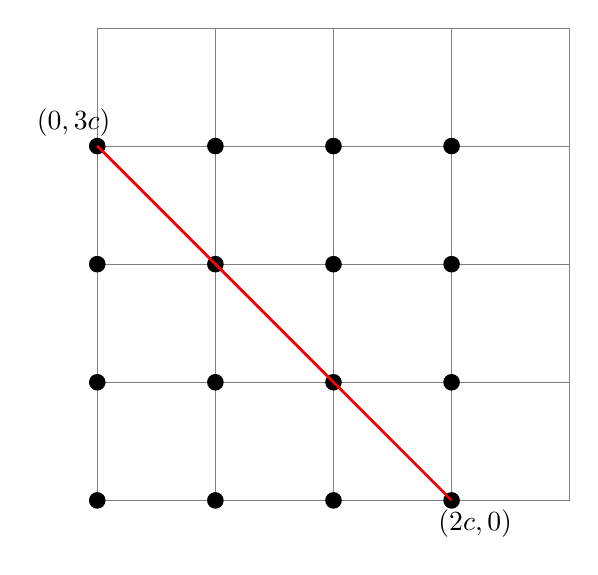
\begin{tikzpicture}[scale=1.5]
    % Draw the grid
    \draw[help lines] (0,0) grid (4,4);
    
    % Draw the points
    \foreach \x in {0,...,3} {
        \foreach \y in {0,...,3} {
            \fill (\x,\y) circle (2pt);
        }
    }
    
    % Draw the black line
    \draw[thick, color=black] (0,3) -- (3,0);
    
    % Draw the red lines
    \draw[thick, color=red] (0,3) -- (2,1);
    \draw[thick, color=red] (0,3) -- (2.5,0.5);
    \draw[thick, color=red] (0,3) -- (3,0);
    
    % Label the points
    \node at (-0.2, 3.2) {$(0,3c)$};
    \node at (3.2, -0.2) {$(2c,0)$};
\end{tikzpicture}

\end{document}